There are many publications demonstrating interesting machine learning algorithms,
features and models to predict efficient program optimizations and hardware
designs~\cite{Monsifrot,SAMP2003,
Marin:2004:CPP:1012888.1005691, SA2005, soffa2005, ABCP06,
CFAP2007, DJBP2009, JGVP2009,
DBLP:conf/cf/ShenVSAS13,DBLP:journals/ijpp/ParkCPBCS13,
DBLP:journals/taco/LeatherBO14,
DBLP:conf/IEEEpact/CumminsP0L17,
Ashouri:2017:MMC:3132652.3124452}.
%
Though all these techniques can be potentially useful, the
lack of common interfaces and meta information for artifacts
and experimental workflows makes it extremely challenging 
to compare, reuse and build upon them particularly 
in industrial projects with tough deadlines.

Even artifact evaluation which we introduced at systems
conferences~\cite{ae} to partially solve these issues is not
yet enough because our community does not have a common, 
portable and customizable workflow framework.
%
Bridging this gap between machine learning and systems research
served as an additional motivation to develop Collective Knowledge
workflow framework.
%
Our idea is to help colleagues and students share various workloads, 
data sets, machine learning algorithms, models and feature extractors 
as plugins (CK modules) with a common API and meta description.
%
Plugged to a common machine learning workflow such modules
can then be applied in parallel to continuously compete 
for the most accurate predictions for a given optimization scenario.
%
Furthermore, the community can continue improving and autotuning models,
analyzing various combination of features, experimenting with hierarchical models, 
and pruning models to reduce their complexity across shared data sets 
to trade off prediction accuracy, speed, size and the ease of interpretation.

   % === CK crowdmodeling ==================================================================
   %CK={"action":"prepare_for_latex", "cid":"slide:a0464dc299d2c8dc", "file":"4d19bcd3cfe164ba-cropped.pdf", "path":"ck-assets", "ck_image":"yes", "ck_image_width":800}
   %CK={"action":"prepare_for_latex", "cid":"slide:a0464dc299d2c8dc", "file":"d2704b9bbf2441c8-cropped.pdf", "path":"ck-assets", "ck_image":"yes", "ck_image_width":800}
   \begin{figure}[!htbp]
     \centering
      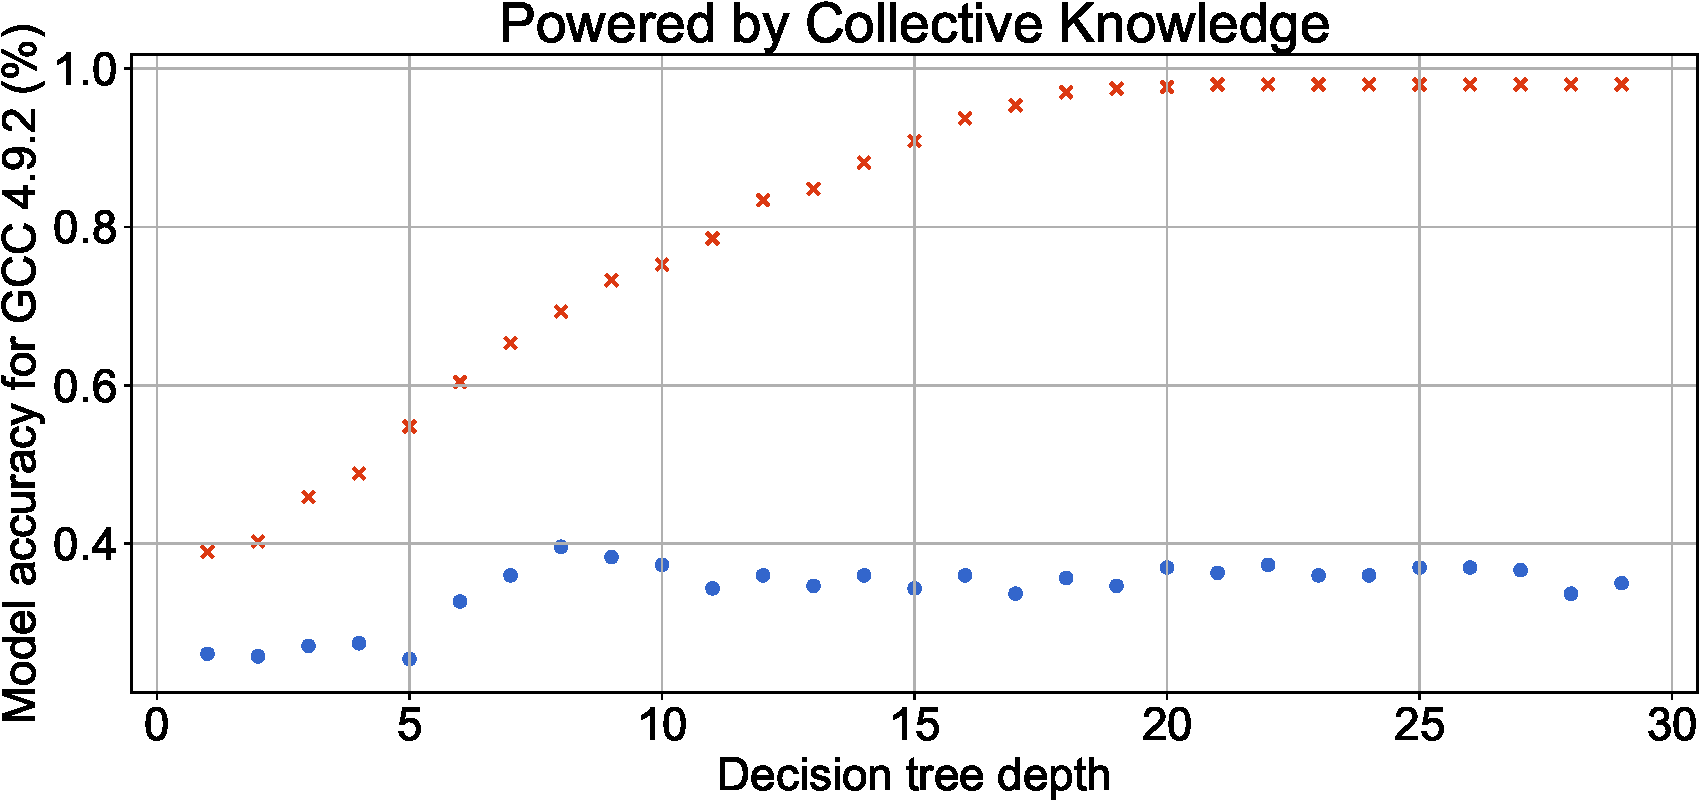
\includegraphics[width=3.2in]
      {ck-assets/4d19bcd3cfe164ba-cropped.pdf} %CK_URL={4d19bcd3cfe164ba-cropped.pdf}
      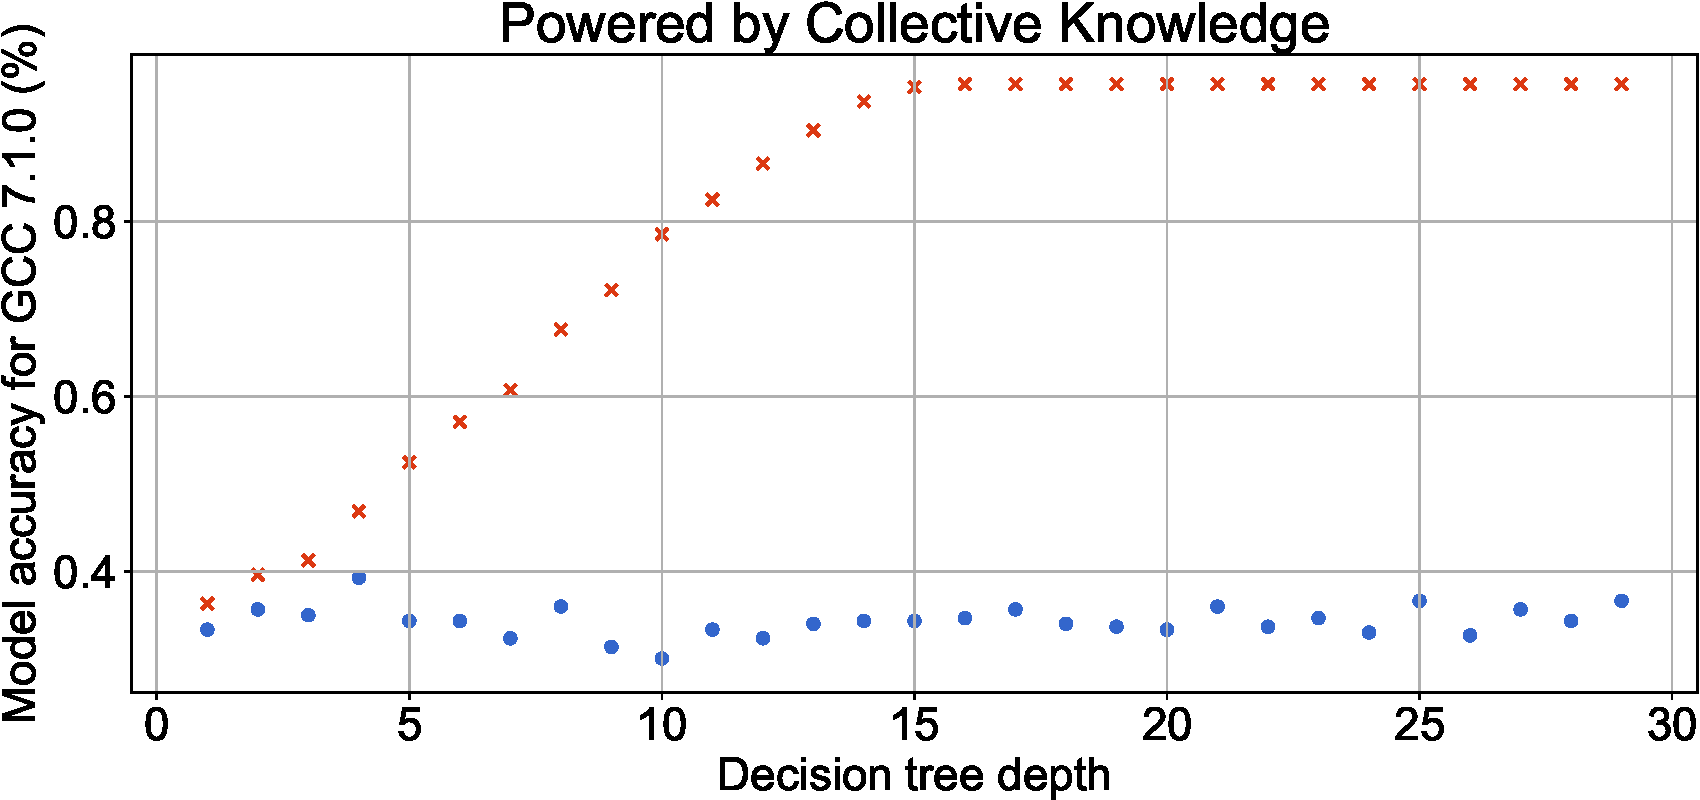
\includegraphics[width=3.2in]
      {ck-assets/d2704b9bbf2441c8-cropped.pdf} %CK_URL={d2704b9bbf2441c8-cropped.pdf}
     \caption{
      Accuracy of an automatically generated decision tree to predict compiler flags (GCC 4.9.2 on the top graph and GCC 7.1.0 on the bottom graph) 
      on RPi3 when autotuning the tree depth.
      Round blue dots show prediction accuracy with cross-validation while blue crosses show
      prediction accuracy without cross-validation.
     }
     \label{fig:ck-model-crowdtuning-gcc}
   \end{figure}

For a proof-of-concept of such collaborative learning approach, 
we shared a number of customizable CK modules (see~\emph{ck search module:*model*})
for several popular classifiers including the nearest neighbor,
decision trees and deep learning.
%
These modules serve as wrappers with a common CK API for
TensorFlow, scikit-learn, R and other machine learning frameworks.
%
We also shared several feature extractors (see \emph{ck search module:*features*}) 
assembling the following groups of program features
which may influence predictions:

\begin{itemize}
  \item {\bf ft1 .. ft56} - original MILEPOST features (see~\cite{29db2248aba45e59:a31e374796869125});
  \item {\bf ft57 .. ft65} - additional features designed and shared by our colleague, Dr. Jeremy Singer~\cite{all-milepost-features};
  \item {\bf ft66 .. ft121} - original MILEPOST features normalized by the total number of instructions (ft24);
\end{itemize}

We then attempted to autotune various parameters
of machine learning algorithms exposed via CK API.
%
Figure~\ref{fig:ck-model-crowdtuning-gcc}
shows an example of autotuning the depth of a decision tree
(available as customizable CK plugin) with all shared groups of features
and its impact on prediction accuracy of compiler flags using MILEPOST
features from the previous section for GCC 4.9.2 and GCC 7.1.0
on RPi3.
%
Blue round dots obtained using leave-one-out validation suggest 
that decision trees of depth 8 and 4 are enough 
to achieve maximum prediction accuracy of 0.4\% for GCC 4.9.2 
and GCC 7.1.0 respectively.
%
Model autotuning thus helped improve prediction accuracy in comparison 
with the original nearest neighbor classifier from the MILEPOST project. 

   % === CK crowdmodeling ==================================================================
   %CK={"action":"prepare_for_latex", "cid":"slide:a0464dc299d2c8dc", "file":"ca86d4d4daf1d84a-cropped.pdf", "path":"ck-assets", "ck_image":"yes", "ck_image_width":300}
   %CK={"action":"prepare_for_latex", "cid":"slide:a0464dc299d2c8dc", "file":"11a3f4efa4479adb-cropped.pdf", "path":"ck-assets", "ck_image":"yes", "ck_image_width":800}
   %CK={"action":"prepare_for_latex", "cid":"slide:a0464dc299d2c8dc", "file":"68deef9c2f07e734-cropped.pdf", "path":"ck-assets", "ck_image":"yes", "ck_image_width":1000}
   \begin{figure*}[!htbp]
     \centering
      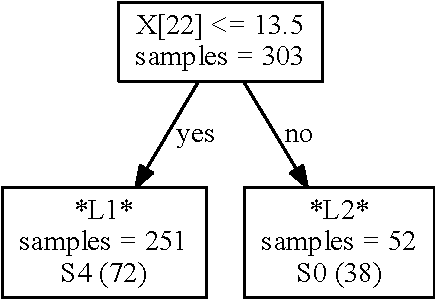
\includegraphics[width=2in]
      {ck-assets/ca86d4d4daf1d84a-cropped.pdf} %CK_URL={ca86d4d4daf1d84a-cropped.pdf}
      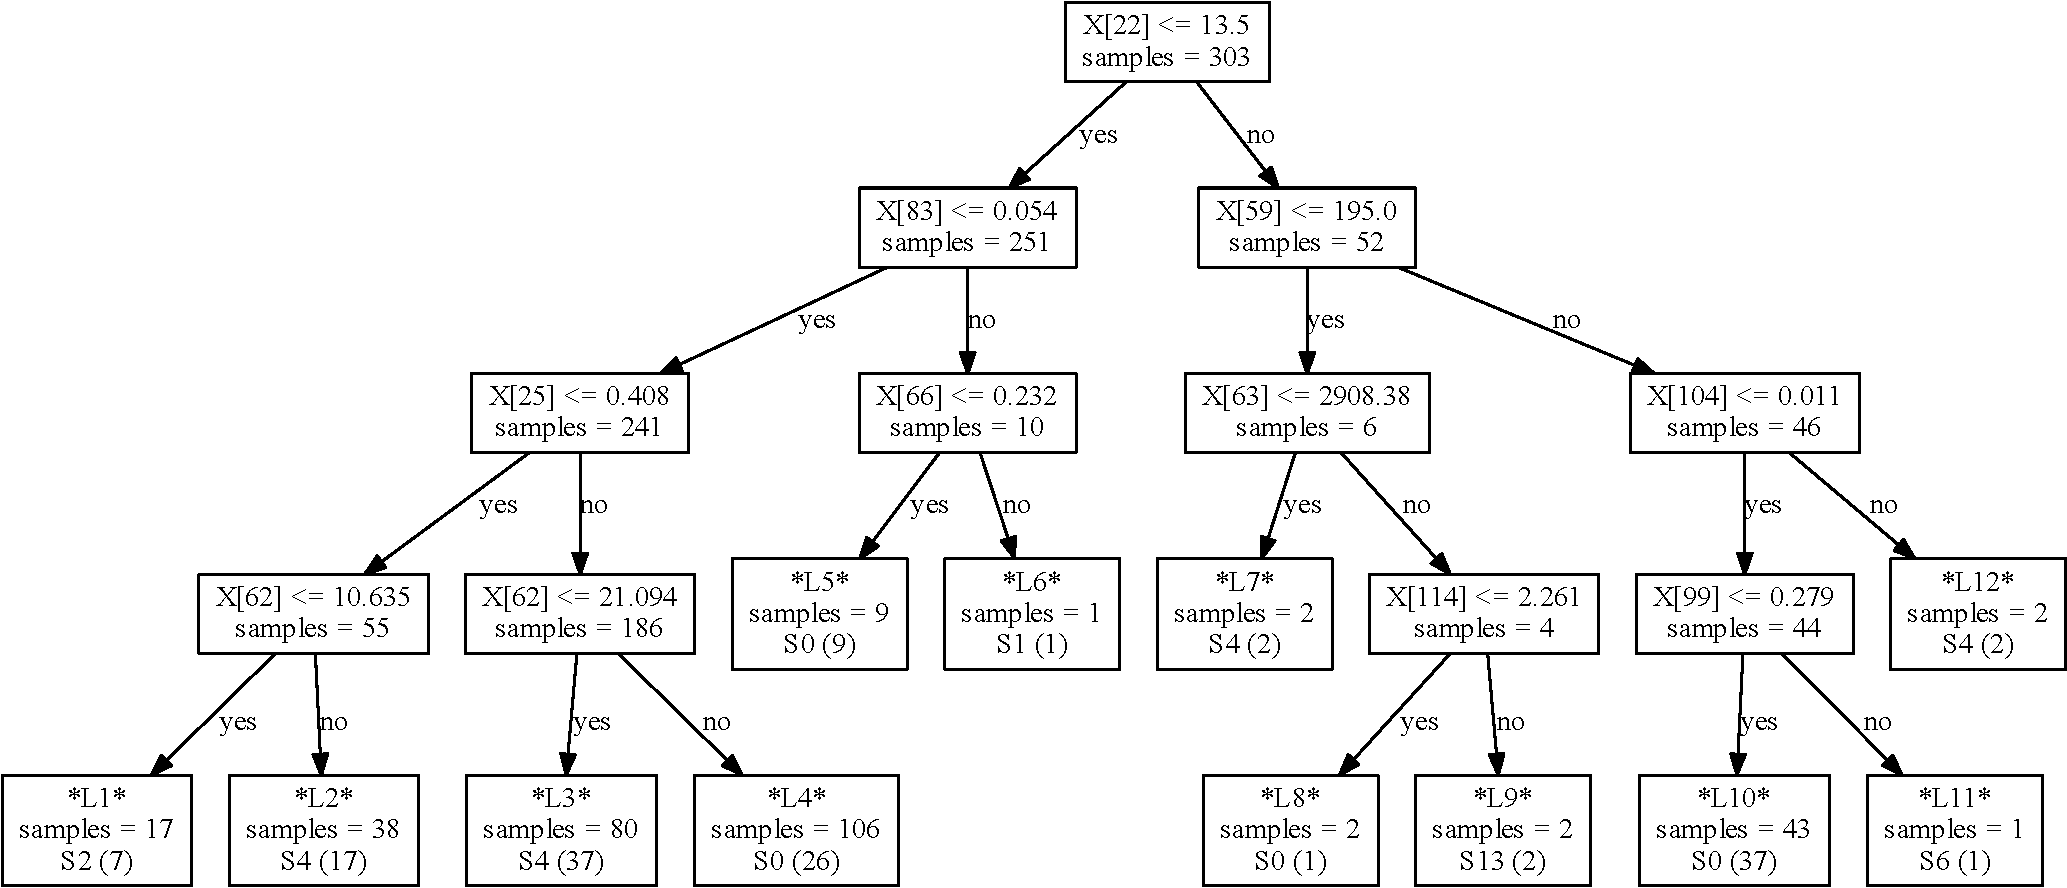
\includegraphics[width=3.6in]
      {ck-assets/11a3f4efa4479adb-cropped.pdf} %CK_URL={11a3f4efa4479adb-cropped.pdf}
      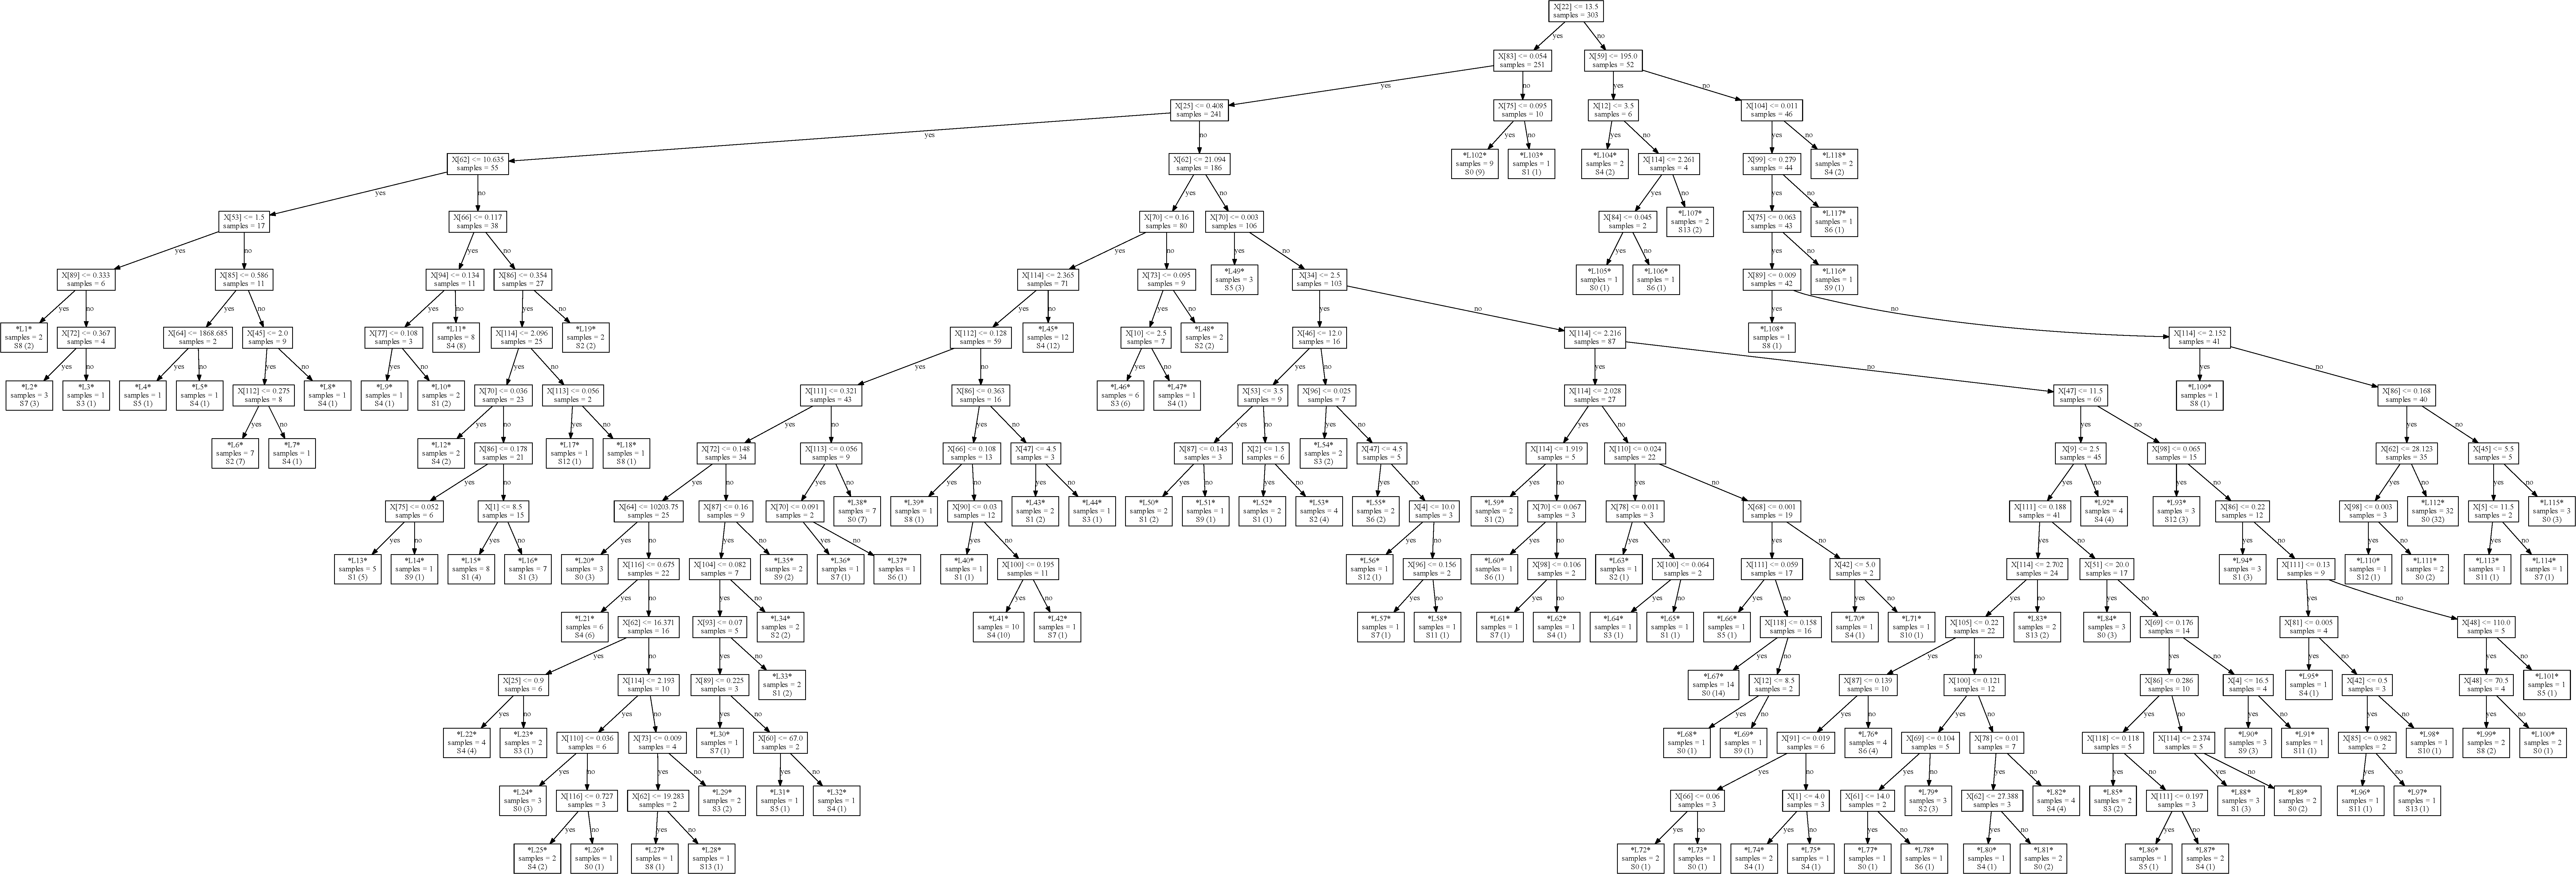
\includegraphics[width=6.6in]
      {ck-assets/68deef9c2f07e734-cropped.pdf} %CK_URL={68deef9c2f07e734-cropped.pdf}
     \caption{
      Example of automatically generated decision trees of depth 1 and 4 with leave-one-out cross-validation, 
      and 15 without cross-validation to predict GCC 7.1.0 compiler optimizations using CK modules.
     }
     \label{fig:ck-model-crowdtuning-gcc7-dt}
   \end{figure*}

Figure~\ref{fig:ck-model-crowdtuning-gcc7-dt} shows a few examples of such automatically
generated decision trees with different depths for GCC 7.1.0 using CK.
%
Such trees are easy to interpret and can therefore help compiler and hardware 
developers quickly understand the most influential features and analyze
relationships between different features and the most efficient
optimizations.
%
For example, the above results suggest that the number of binary integer operations (ft22) 
and the number of distinct operators (ft59) can help predict optimizations 
which can considerably improve execution time of a given method over -O3.

Turning off cross-validation can also help developers understand 
how well models can perform on all available workloads (in-sample data)
(red dots on Figure~\ref{fig:ck-model-crowdtuning-gcc}).
%
In our case of GCC 7.1.0, the decision tree of depth 15 shown in Figure~\ref{fig:ck-model-crowdtuning-gcc7-dt})
is enough to capture all compiler optimizations for ~300 available workloads.

  % === all model results ==================================================================
  %CK={"action":"prepare_for_latex", "cid":"slide:a0464dc299d2c8dc", "file":"74089e922ca45f99-table.tex", "uid":"defbc62fc4d1fa78", "path":"ck-assets"}
  %CK={"action":"prepare_for_latex", "cid":"slide:a0464dc299d2c8dc", "file":"142fbaf8c4fb48b8-table.tex", "uid":"defbc62fc4d1fa78", "path":"ck-assets"}
  %CK={"action":"prepare_for_latex", "cid":"slide:a0464dc299d2c8dc", "file":"74089e922ca45f99-table.html", "uid":"defbc62fc4d1fa78", "path":"ck-assets"}
  \begin{table*}[!htbp]
    \centering
    {\small
         \begin{tabular}{|l|p{1.2in}|p{0.9in}|p{0.9in}|}
     \hline
      \textbf{Model} & \textbf{Features} & \textbf{Accuracy (GCC 4.9.2)} & \textbf{Accuracy (GCC 7.1.0)} \\ 
     \hline
      \textbf{ decision trees with cross validation; depth 1 } &  ft1 .. ft65  &  0.26  &  0.33 \\
     \hline
      \textbf{ decision trees with cross validation; depth 2 } &  ft1 .. ft65  &  0.26  &  0.36 \\
     \hline
      \textbf{ decision trees with cross validation; depth 4 } &  ft1 .. ft65  &  0.27  &  0.39 \\
     \hline
      \textbf{ decision trees with cross validation; depth 8 } &  ft1 .. ft65  &  0.40  &  0.36 \\
     \hline
      \textbf{ decision trees with cross validation; depth 16 } &  ft1 .. ft65  &  0.36  &  0.35 \\
     \hline
      \textbf{ decision trees with cross validation; depth 20 } &  ft1 .. ft65  &  0.37  &  0.33 \\
     \hline
      \textbf{ decision trees with cross validation; depth 25 } &  ft1 .. ft65  &  0.37  &  0.37 \\
     \hline
      \textbf{ decision trees with cross validation; depth 29 } &  ft1 .. ft65  &  0.35  &  0.37 \\
     \hline
      \textbf{ decision trees without cross validation; depth 1 } &  ft1 .. ft65  &  0.39  &  0.36 \\
     \hline
      \textbf{ decision trees without cross validation; depth 2 } &  ft1 .. ft65  &  0.40  &  0.40 \\
     \hline
      \textbf{ decision trees without cross validation; depth 4 } &  ft1 .. ft65  &  0.49  &  0.47 \\
     \hline
      \textbf{ decision trees without cross validation; depth 8 } &  ft1 .. ft65  &  0.69  &  0.68 \\
     \hline
      \textbf{ decision trees without cross validation; depth 16 } &  ft1 .. ft65  &  0.94  &  0.96 \\
     \hline
      \textbf{ decision trees without cross validation; depth 20 } &  ft1 .. ft65  &  0.98  &  0.96 \\
     \hline
      \textbf{ decision trees without cross validation; depth 25 } &  ft1 .. ft65  &  0.98  &  0.96 \\
     \hline
      \textbf{ decision trees without cross validation; depth 29 } &  ft1 .. ft65  &  0.98  &  0.96 \\
     \hline
      \textbf{ dnn tf with cross validation; iteration 1 } &  ft1 .. ft65  &  0.68  &  0.30 \\
     \hline
      \textbf{ dnn tf with cross validation; iteration 2 } &  ft1 .. ft65  &  0.64  &  0.33 \\
     \hline
      \textbf{ dnn tf with cross validation; iteration 3 } &  ft1 .. ft65  &  0.61  &  0.45 \\
     \hline
      \textbf{ dnn tf with cross validation; iteration 4 } &  ft1 .. ft65  &  0.64  &  0.44 \\
     \hline
      \textbf{ dnn tf without cross validation; iteration 1 } &  ft1 .. ft65  &  0.72  &  0.29 \\
     \hline
      \textbf{ dnn tf without cross validation; iteration 2 } &  ft1 .. ft65  &  0.72  &  0.47 \\
     \hline
      \textbf{ dnn tf without cross validation; iteration 3 } &  ft1 .. ft65  &  0.72  &  0.48 \\
     \hline
      \textbf{ dnn tf without cross validation; iteration 4 } &  ft1 .. ft65  &  0.68  &  0.62 \\
     \hline
      \textbf{ milepost nn } &  ft1 .. ft121  &  0.30  &  0.30 \\
     \hline
      \textbf{ milepost nn } &  ft1 .. ft56  &  0.37  &  0.30 \\
     \hline
      \textbf{ milepost nn } &  ft1 .. ft65  &  0.30  &  0.30 \\
     \hline
      \textbf{ milepost nn } &  ft57 .. ft121  &  0.30  &  0.30 \\
     \hline
      \textbf{ milepost nn } &  ft57 .. ft65  &  0.30  &  0.30 \\
     \hline
      \textbf{ milepost nn } &  ft66 .. ft121  &  0.36  &  0.32 \\
     \hline
      \textbf{ milepost nn } &  ft1 .. ft121\newline(normalized)  &  0.37  &  0.37 \\
     \hline
      \textbf{ milepost nn } &  ft1 .. ft56\newline(normalized)  &  0.37  &  0.33 \\
     \hline
      \textbf{ milepost nn } &  ft1 .. ft65\newline(normalized)  &  0.39  &  0.32 \\
     \hline
      \textbf{ milepost nn } &  ft57 .. ft121\newline(normalized)  &  0.37  &  0.39 \\
     \hline
      \textbf{ milepost nn } &  ft57 .. ft65\newline(normalized)  &  0.37  &  0.35 \\
     \hline
      \textbf{ milepost nn } &  ft66 .. ft121\newline(normalized)  &  0.38  &  0.38 \\
     \hline
      \textbf{ milepost nn (reduce complexity1) } &  ft1 .. ft121\newline(normalized)  &  0.45  &  0.44 \\
     \hline
      \textbf{ milepost nn (reduce complexity2) } &  ft1 .. ft121\newline(normalized)  &  0.45  &  0.40 \\
     \hline
    \end{tabular}     %CK_HTML={ck-assets/74089e922ca45f99-table.html}
    }
    \caption{
     Prediction accuracy when autotuning or reducing complexity of decision tree, 
     nearest neighbor and deep learning classifiers
     across different groups of program features.
    }
    \label{fig:crowdmodeling-all-rpi3-progs}
  \end{table*}

To complete our demonstration of CK concepts for collaborative machine learning and optimization,
we also evaluated a deep learning based classifier from TensorFlow~\cite{DBLP:journals/corr/AbadiABBCCCDDDG16}
(see \emph{ck help module:model.tf})
with 4 random configurations of hidden layers ([10,20,10], [21,13,21], [11,30,18,20,13], [17]) 
and training steps (300..3000).
%
We also evaluated the nearest neighbor classifier used in the MILEPOST project but with different groups of features 
and aggregated all results in Table~\ref{fig:crowdmodeling-all-rpi3-progs}. 
%
Finally, we automatically reduced the complexity of the nearest neighbor classifier (1) by iteratively removing those features one by one
which do not degrade prediction accuracy and (2) by iteratively adding features one by one to maximize prediction accuracy.
%
It is interesting to note that our nearest neighbor classifier achieves
a slightly better prediction accuracy with a reduced feature set than with 
a full set of features showing inequality of MILEPOST features
and overfitting.

As expected, deep learning classification achieves a better prediction accuracy of 0.68\%
and 0.45\% for GCC 4.9.2 and GCC 7.1.0 respectively for RPi3 among currently shared models, 
features, workloads and optimizations.
%
However, since deep learning models are so much more computationally intensive, resource hungry
and difficult to interpret than decision trees, one must carefully balance accuracy vs speed vs size.
%
That is why we suggest to use hierarchical models where
high-level and coarse-grain program behavior is quickly captured 
using decision trees, while all fine-grain behavior is captured 
by deep learning and similar techniques.
%
Another possible use of deep learning can be in automatically capturing
influential features from the source code, data sets and hardware.

\textit{All scripts to generate above experiments (require further documentation)
are available in the following CK entry:}

\begin{flushleft}
\texttt{\$ ck find script:rpi3-crowdmodel}
\end{flushleft}
